\documentclass[11pt,a4paper,twocolumn]{article}

% === Core Packages ===
\usepackage[margin=2cm]{geometry}
\usepackage[utf8]{inputenc}
\usepackage[T1]{fontenc}
\usepackage{times}
\usepackage{amsmath,amssymb}
\usepackage{graphicx}
\usepackage{booktabs}
\usepackage{float}
\usepackage{enumitem}
\usepackage{tikz}
\usepackage{pgfplots}
\pgfplotsset{compat=1.18}
\usetikzlibrary{arrows.meta,shapes.geometric,positioning,calc,decorations.markings,fit,backgrounds}

% === Citation (IEEE style) ===
\usepackage[numbers,sort&compress]{natbib}
\bibliographystyle{IEEEtranN}

% === Hyperref ===
\usepackage[hidelinks]{hyperref}
\usepackage{xurl}

% === Settings ===
\setlength{\parindent}{1em}
\setlength{\parskip}{0.3em}

% === Title ===
\title{\textbf{Rețea Descentralizată de Reputație:\\Un cadru pentru organizarea socială naturală}}
\author{Pavel Kudrna\\Prague, Czechia\\Draft v1 --- March 2026}
\date{}

\begin{document}
\maketitle

% ============================================================
% ABSTRACT
% ============================================================
\begin{abstract}
Simțul dreptății---convingerea că nedreptățile sunt îndreptate și meritul este răsplătit---este cea mai puternică forță de coeziune a societății. Când instituțiile centralizate de guvernare nu pot oferi acest simț pentru că nivelul costului impunerii unui drept depășește valoarea dreptului însuși, coeziunea socială se erodează. Structurile instituționale actuale eșuează în a soluționa o categorie semnificativă de dispute în același mod sistematic în care planificarea centralizată eșuează în alocarea resurselor: prin asimetrie informațională, bucle de feedback lipsă și deconectarea decidenților de consecințele deciziilor lor. Această lucrare prezintă o Rețea Socială de Reputație (RSN): un strat de comunicare descentralizat, incoruptibil și rezistent la cenzură, construit pe Identificatori Descentralizați (DID), care permite participanților pseudonimi să publice, să verifice și să consume informații de reputație despre comportamentul din lumea reală. Mecanismul central se bazează pe trei principii de proiectare: (1)~o structură asimetrică a costurilor în care citirea datelor de reputație este ieftină, dar scrierea necesită efort verificabil; (2)~un protocol nedeterminist de selecție a verificatorilor bazat pe hashing consistent, care taxează afirmațiile radicale prin costuri de iterație în creștere; și (3)~un model de autoritate de reputație orientat spre piață, în care verificatorii privați își pun în joc reputația acumulată pe acuratețea afirmațiilor pe care le avizează. Arhitectura rezultată produce o meritocrație emergentă fără coordonare centrală și permite o cale de migrare graduală și reversibilă de la sistemele existente administrate de stat.
\end{abstract}

% ============================================================
% 1. INTRODUCTION
% ============================================================
\section{Introducere}

\subsection{Problema încrederii centralizate}

Guvernarea modernă se sprijină pe o presupunere fundamentală: că instituțiile centralizate pot media încrederea între străini la scară largă. Instanțele soluționează disputele. Registrele certifică proprietatea. Organismele de reglementare impun standarde. Aceste instituții au fost concepute într-o epocă în care informația era rară, comunicarea era lentă, iar delegarea autorității către un organism central era singurul mecanism de coordonare fezabil. Guvernarea centralizată eșuează însă din aceleași motive structurale ca și planificarea centralizată: asimetrie informațională, bucle de feedback lipsă și deconectarea decidenților de consecințele deciziilor lor.

Presupunerea eșuează, de exemplu, atunci când costul medierii instituționale depășește valoarea disputei. Să considerăm un chiriaș care descoperă că apartamentul închiriat nu are un certificat de siguranță electrică cerut de lege---o condiție care reprezintă un pericol imediat pentru viață. Dreptul legal al chiriașului de a se retrage din contract este neechivoc. Totuși, costul impunerii acestui drept prin sistemul judiciar depășește valoarea monetară a garanției și a daunelor datorate, chiar incluzând eventualele compensații statutare~\cite{czcourtfees}. Răspunsul rațional este să absoarbă pierderea și să iasă.

Acesta nu este un caz-limită patologic. Este experiența implicită pentru o categorie semnificativă de dispute în care prejudiciul este real, dar mizele monetare se situează sub pragul la care impunerea instituțională devine rațională din punct de vedere economic. Rezultatul este un sistem care favorizează structural actorii răuvoitori: cei care aduc prejudicii altora în volume sub acest prag pot acționa în impunitate, deoarece costul căutării dreptății cade asupra părții vătămate.

Exemplul de mai sus provine din mediul juridic al autorului---sistemul de drept civil ceh. În alte tradiții juridice---dreptul comun bazat pe precedent, dreptul cutumiar, sistemele mixte---dreptatea eșuează în moduri diferite și în grade diferite, în funcție de specificul cultural și procedural al jurisdicției. Cititorii vor recunoaște probabil exemple echivalente din propriul context. Ceea ce este universal din punct de vedere structural este tiparul: disputele a căror valoare cade sub pragul impunerii raționale economic se încheie cu pierderea absorbită de partea vătămată. RSN nu promite o dreptate perfectă---doar reduce avantajul structural de care se bucură actorii răuvoitori atunci când impunerea instituțională este neeconomică.

\subsection{De ce soluțiile existente sunt insuficiente}

\textbf{Cadrele de identitate descentralizată (DID)}~\cite{did2022} oferă mecanisme criptografice pentru gestionarea identității suverane a sinelui, dar se concentrează în primul rând pe verificarea identității, fără a aborda întrebarea mai amplă a reputației comportamentale.

\textbf{Token-urile Soulbound (SBT)}~\cite{weyl2022} surprind ideea că reputația este netransferabilă, dar se bazează pe infrastructură blockchain cu constrângeri de scalabilitate și nu abordează stimulentele economice care guvernează introducerea informației. Concepte înrudite precum token-urile de merit (de ex., Liberland) împărtășesc o filozofie similară, dar rămân legate de cadre jurisdicționale specifice.

\textbf{Organizațiile Autonome Descentralizate (DAO)}~\cite{buterin2014} implementează guvernarea prin contracte inteligente, dar reproduc dinamici plutocratice în care influența este proporțională cu capitalul. Votul cuadratic~\cite{buterin2019} atenuează parțial acest lucru, dar limitează adoptarea practică. DAO-urile se confruntă de asemenea cu \emph{problema oracolului} fundamentală: contractele inteligente nu pot verifica în mod fiabil stările din lumea reală fără o sursă externă de încredere, iar această problemă nu are o soluție generală în cadrul arhitecturii blockchain.

Niciun sistem existent nu combină descentralizarea, rezistența la cenzură, pseudonimitatea, costul verificabil de intrare și consensul emergent.

\subsection{Contribuții}

Această lucrare aduce următoarele contribuții:
\begin{enumerate}[nosep]
\item Definirea \textbf{Rețelei Sociale de Reputație (RSN)}, un protocol descentralizat care extinde cadrul DID pentru a susține schimbul bilateral de reputație.
\item Un \textbf{protocol nedeterminist de selecție a verificatorilor} bazat pe hashing consistent~\cite{karger1997}.
\item \textbf{Principiul Radicalismului Costisitor}, care taxează afirmațiile în funcție de distanța lor față de consensul rețelei prin trei canale de cost care se compun.
\item Un \textbf{model de Autoritate Reputabilă} cu stimulente asimetrice, în care avizarea falsă costă catastrofal mai mult decât onorariile legitime.
\item O \textbf{cale de migrare graduală} printr-o infrastructură fiscală paralelă.
\end{enumerate}

% ============================================================
% 2. DESIGN PRINCIPLES
% ============================================================
\section{Principii de proiectare}

Arhitectura RSN este constrânsă de cinci principii de proiectare nenegociabile.

\textbf{Continuitate și evoluție.} Sistemul coexistă cu instituțiile existente pe parcursul unei perioade de tranziție de durată nedeterminată. Tranziția trebuie să fie reversibilă în fiecare etapă.

\textbf{Voluntariat și responsabilitate.} Participarea este voluntară, dar voluntariatul este cuplat cu responsabilitatea: un participant care preia controlul asupra unei funcții instituționale își asumă simultan obligațiile aferente.

\textbf{Diversitate și neutralitate culturală.} Consensul emerge din interacțiuni bilaterale, nu din reguli prestabilite impuse de proiectanții sistemului.

\textbf{Reziliență și rezistență la cenzură.} Costul cenzurării rețelei trebuie să depășească costul tolerării ei. Doar totalitarismul deplin---cu un cost politic și economic ruinător---poate suprima sistemul.

\textbf{Consens și impunere.} Sistemul încorporează tendințele umane spre meschinărie, ranchiună și satisfacție retributivă ca trăsături de rezistență structurală. Reaua conduită nu este interzisă; ea este taxată.

% ============================================================
% 3. SYSTEM OVERVIEW
% ============================================================
\section{Prezentare generală a sistemului}

\subsection{Rețeaua Socială de Reputație}

RSN este un strat de comunicare descentralizat, peer-to-peer, în care participanții schimbă informații verificabile despre comportamentul din lumea reală. Proprietățile sale definitorii sunt: infrastructură descentralizată și necenzurabilă; participare pseudonimă prin DID-uri; structură asimetrică a costurilor (citirea este ieftină, scrierea este costisitoare); verificabilitate criptografică; și \textbf{suport pentru standarde}---formate care pot fi citite de mașini pentru informația propagată prin rețea, pentru serviciile oferite de autorități (compunerea afirmațiilor, avizarea, serviciul de martor) și pentru formatul de politică, incluzând reguli de evaluare a reputației contrapărții și de estimare a riscului de nepotrivire a politicii (între comportamentul declarat și cel real).

\subsection{Componente arhitecturale}

RSN constă din patru componente principale (Fig.~\ref{fig:architecture}):
\begin{enumerate}[nosep]
\item \textbf{Stratul DID.} Identitățile participanților cu reguli declarate, metadate de reputație și rutare de rețea.
\item \textbf{Protocolul de afirmații.} Format structurat pentru publicarea de aserțiuni despre evenimente din lumea reală.
\item \textbf{Rețeaua de verificare.} Protocol descentralizat pentru atribuirea verificatorilor folosind hashing consistent.
\item \textbf{Stratul de agregare a reputației.} Servicii care produc rezumate de reputație lizibile pentru oameni.
\end{enumerate}

\begin{figure}[ht]
\centering
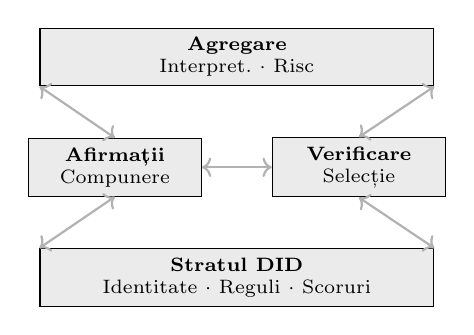
\begin{tikzpicture}[
    layer/.style={draw, minimum height=0.7cm, align=center, font=\scriptsize, fill=black!8},
    arr/.style={<->, thick, gray!60}
]
\node[layer, minimum width=5cm] (agg) at (0,2.8) {\textbf{Agregare}\\Interpret.\ $\cdot$ Risc};
\node[layer, minimum width=2.2cm] (claim) at (-1.55,1.4) {\textbf{Afirmații}\\Compunere};
\node[layer, minimum width=2.2cm] (verif) at (1.55,1.4) {\textbf{Verificare}\\Selecție};
\node[layer, minimum width=5cm] (did) at (0,0) {\textbf{Stratul DID}\\Identitate $\cdot$ Reguli $\cdot$ Scoruri};

\draw[arr] (agg.south west) -- (claim.north);
\draw[arr] (agg.south east) -- (verif.north);
\draw[arr] (claim.east) -- (verif.west);
\draw[arr] (claim.south) -- (did.north west);
\draw[arr] (verif.south) -- (did.north east);
\end{tikzpicture}
\caption{Arhitectura RSN pe patru straturi.}
\label{fig:architecture}
\end{figure}

\subsection{Rolurile participanților}

O tranzacție de verificare implică până la șase roluri DID distincte (Fig.~\ref{fig:roles}): \textbf{Emitentul} ($DID_I$, creează și trimite afirmația), \textbf{Subiectul} ($DID_S$, DID-ul despre care este afirmația---poate coincide cu Emitentul), \textbf{Autoritatea} ($DID_A$, avizează afirmația contra unui onorariu; poate oferi și servicii de martor---\emph{opțional}), \textbf{Martorul} ($DID_{W_{1..n}}$, monitor incognito al onestității verificatorului prin coduri de provocare---\emph{opțional}), \textbf{Verificatorul} ($DID_V$, selectat algoritmic pentru a publica afirmația) și \textbf{RSN} (rețeaua în care sunt publicate afirmațiile verificate). Orice rol poate fi delegat unui alt DID (Secțiunea~7.4). O Autoritate combină în mod obișnuit avizarea cu serviciile de martor, dar cele două funcții sunt logic independente.

\begin{figure}[ht]
\centering
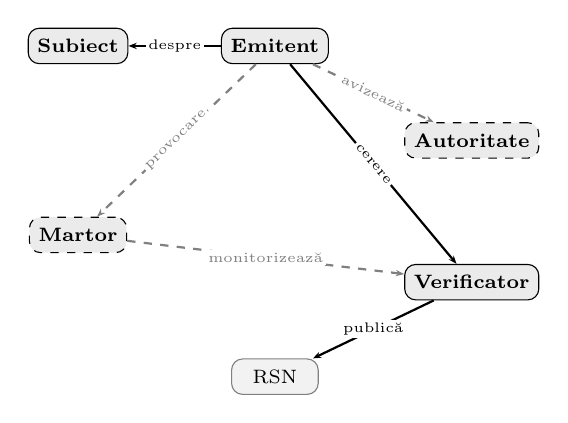
\begin{tikzpicture}[
    role/.style={draw, rounded corners, minimum width=1.1cm, minimum height=0.45cm, align=center, font=\scriptsize, fill=black!8},
    opt/.style={draw, rounded corners, minimum width=1.1cm, minimum height=0.45cm, align=center, font=\scriptsize, fill=black!8, dashed},
    arr/.style={-{Stealth[length=3pt]}, thick},
    oarr/.style={-{Stealth[length=3pt]}, thick, dashed, gray},
    lbl/.style={font=\tiny, fill=white, inner sep=1pt}
]
\node[role] (I) at (0,2.4) {\textbf{Emitent}};
\node[role] (S) at (-2.5,2.4) {\textbf{Subiect}};
\node[opt] (A) at (2.5,1.2) {\textbf{Autoritate}};
\node[opt] (W) at (-2.5,0) {\textbf{Martor}};
\node[role] (V) at (2.5,-0.6) {\textbf{Verificator}};
\node[role, fill=black!5, draw=gray] (N) at (0,-1.8) {RSN};

\draw[arr] (I) -- node[lbl] {despre} (S);
\draw[oarr] (I) -- node[lbl,sloped] {avizează} (A);
\draw[oarr] (I) -- node[lbl,sloped] {provocare} (W);
\draw[arr] (I) -- node[lbl,sloped] {cerere} (V);
\draw[oarr] (W) -- node[lbl] {monitorizează} (V);
\draw[arr] (V) -- node[lbl] {publică} (N);
\end{tikzpicture}
\caption{Rolurile DID într-o tranzacție de verificare. Linie punctată = opțional (Autoritate, Martor).}
\label{fig:roles}
\end{figure}

\subsection{Incoruptibilitate: patru forțe}

Incoruptibilitatea RSN nu provine dintr-un singur mecanism, ci din patru forțe concurente. Niciuna nu este suficientă în sine; doar combinația lor face ca o tentativă de corupere să fie irațională din punct de vedere economic.

\textbf{Țintă imprevizibilă.} Verificatorul pentru fiecare afirmație este selectat nedeterminist prin hashing consistent (Secțiunea~5.3). Un atacator nu poate viza în prealabil un verificator anume pentru mituire, deoarece identitatea verificatorului este o funcție a conținutului afirmației și a iterațiilor anterioare, nu a alegerii emitentului.

\textbf{Efect de pârghie reputațional---creștere lentă, prăbușire rapidă.} Reputația poate fi câștigată doar incremental, printr-un comportament consistent susținut. Ea poate fi însă pierdută catastrofal printr-o singură avizare frauduloasă (Secțiunea~6.2). Această asimetrie înseamnă că ani de reputație acumulată pot fi distruși de o singură avizare necinstită; strategia optimă rămâne respingerea afirmațiilor suspecte.

\textbf{Promisiune publică.} Fiecare Deținător de DID își declară public politica---un set de reguli care pot fi citite de mașini pe care se angajează să le urmeze. Divergența dintre declarație și comportamentul real este detectabilă și taxată ca o abatere reputațională mai gravă decât încălcarea de bază (Secțiunea~7.3). Ipocrizia este, prin urmare, mai costisitoare decât necinstea directă.

\textbf{Asimetria costului atacului asupra rețelei mesh.} Costul cenzurării sau destabilizării rețelei crește neliniar odată cu dimensiunea și densitatea rețelei, în timp ce costul tolerării ei rămâne constant. Pentru ca cenzura să merite, un actor centralizat ar trebui să o aplice pe întreaga rețea---necesitând măsuri disproporționate față de orice beneficiu imaginabil (Secțiunea~10).

% ============================================================
% 4. DECENTRALIZED IDENTITY MODEL
% ============================================================
\section{Modelul de identitate descentralizată}

\subsection{DID cu proprietăți speciale}

RSN extinde specificația W3C DID Core~\cite{did2022} cu: \textbf{Reguli declarate} (angajamente comportamentale care pot fi citite de mașini), \textbf{Metadate de reputație} (scor comportamental agregat) și \textbf{Rutare de rețea} (poartă onion mutabilă, separată de poziția stabilă pe inel).

\subsection{Ciclul de viață al afirmației}

O Afirmație parcurge șase etape (Fig.~\ref{fig:lifecycle}): compunere, avizare opțională de către autoritate, selecția verificatorului prin hashing consistent, decizia de verificare (acceptare sau respingere cu iterație), publicare și actualizarea reputației pentru toate părțile.

\begin{figure}[ht]
\centering
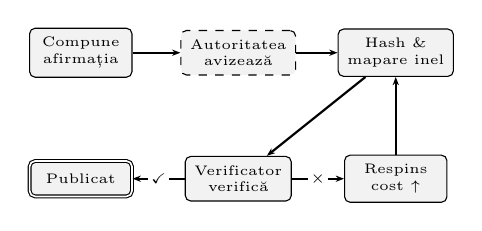
\begin{tikzpicture}[
    stp/.style={draw, rounded corners=2pt, minimum width=1.3cm, minimum height=0.45cm, align=center, font=\tiny, fill=black!5},
    arr/.style={-{Stealth[length=3pt]}, thick},
    lbl/.style={font=\tiny, fill=white, inner sep=1pt}
]
\node[stp] (comp) at (0,0) {Compune\\afirmația};
\node[stp, dashed] (auth) at (2.0,0) {Autoritatea\\avizează};
\node[stp] (hash) at (4.0,0) {Hash \&\\mapare inel};
\node[stp] (ver) at (2.0,-1.6) {Verificator\\verifică};
\node[stp, double] (pub) at (0,-1.6) {Publicat};
\node[stp] (rej) at (4.0,-1.6) {Respins\\cost $\uparrow$};

\draw[arr] (comp) -- (auth);
\draw[arr] (auth) -- (hash);
\draw[arr] (hash) -- (ver);
\draw[arr] (ver) -- node[lbl] {\checkmark} (pub);
\draw[arr] (ver) -- node[lbl] {$\times$} (rej);
\draw[arr] (rej) -- ++(0,0.8) -| (hash);
\end{tikzpicture}
\caption{Ciclul de viață al afirmației cu bucla de iterație.}
\label{fig:lifecycle}
\end{figure}

\subsection{Relația cu W3C DID Core}

Modelul de identitate al RSN este un supraset propriu al specificației W3C DID Core~\cite{did2022}. Toate DID-urile RSN sunt DID-uri W3C valide. Extensiile specifice RSN sunt codificate ca proprietăți ale documentului DID, definite într-o specificație de metodă DID dedicată, compatibilă cu infrastructura existentă precum ION~\cite{buchner2021} și Ceramic~\cite{ceramic2023}.

% ============================================================
% 5. VERIFICATION AND PROPAGATION
% ============================================================
\section{Verificarea și propagarea informației}

\subsection{Costul intrării informației}

Principiul economic central al RSN este asimetria dintre citire și scriere. Citirea datelor de reputație se apropie de un cost marginal zero pentru participanții care fac parte din rețeaua DID și au acces proporțional cu reputația lor---noii veniți trebuie să câștige treptat un acces mai larg (vezi anti-parazitismul). Scrierea---înțeleasă ca materializarea durabilă a reputației în rețea, nu ca un act tehnic punctual---necesită o investiție cumulativă verificabilă pe trei dimensiuni: \textbf{timp} (ani de viață dedicați comportamentului consistent, angajamentelor onorate și relațiilor cultivate), \textbf{energie} (efort investit în tranzacții oneste, grija pentru parteneriate și fiabilitate pe termen lung) și \textbf{bani} (investiție în propriul nume---dezvoltare profesională, calitatea muncii, reparații pentru prejudiciile cauzate). Reputația nu poate fi cumpărată instantaneu---este rezultatul unei acumulări de-o viață pe care sistemul doar o face vizibilă și transferabilă între contexte. Costurile tehnice punctuale ale protocolului (semnături criptografice, onorarii ale verificatorilor) sunt neglijabile în comparație cu această investiție de bază.

\subsection{Graful social și profunzimea contactelor}

RSN este fundamental o rețea socială: fiecare DID adaugă contacte (alte DID-uri) care permit conexiunea. Aceste contacte au propriile lor contacte, și așa mai departe. Căutarea algoritmică a verificatorului operează în interiorul unei profunzimi configurabile $h$ de contacte legate (de ex., $h=3$: contactele directe, contactele lor și contactele contactelor). Această arhitectură nu necesită un singur blockchain global---favorizează în mod natural emergența unor comunități/clustere cu suprapuneri către alte comunități. Fiecare participant DID trebuie să aibă o \textbf{politică} publicată---un set de reguli care pot fi citite de mașini care guvernează modul în care sunt evaluate cererile primite. Încălcările de politică sunt înregistrate în rețea ca artefacte negative.

\subsection{Selecția algoritmică a verificatorului}

Protocolul de verificare folosește hashing consistent~\cite{karger1997} (Fig.~\ref{fig:verifier}). Verificarea este un serviciu contra cost: verificatorii operează pentru un onorariu, creând o piață în care concurența determină prețul, viteza și fiabilitatea.

\textbf{Pasul 1.} Documentul afirmației este concatenat cu rezultatul hash al iterației anterioare (sau $\varnothing$ la prima iterație) și hash-uit:
\begin{equation}
\text{pos} = f_h(\text{claim} \| \text{prev\_hash})
\label{eq:hash}
\end{equation}

Algoritmul trebuie să includă \emph{calea completă} a tuturor cererilor și răspunsurilor anterioare---nu doar un hash al iterației precedente. Răspunsul complet al fiecărui verificator (acceptare, respingere, preț cotat, motiv) este adăugat documentului în creștere, verificabil prin semnături criptografice la fiecare pas.

\textbf{Pasul 2.} Hash-ul este mapat pe $N$ poziții pe inelul de hashing consistent, distribuite uniform (de ex., pentru $N=4$: $+0^{\circ}, +90^{\circ}, +180^{\circ}, +270^{\circ}$). Din fiecare poziție, o căutare în sensul acelor de ceasornic selectează cel mai apropiat DID drept candidat verificator (Fig.~\ref{fig:multipoint}). $N$ este un parametru variabil care poate depinde de procentul de DID-uri active la momentul respectiv, de ora din zi sau de reactivitatea istorică a rețelei.

\textbf{Pasul 3.} Verificatorul acceptă (publică, punându-și în joc reputația) sau respinge (revenind la Pasul~1 cu hash-ul respingerii). Când un nod nu răspunde deși declară statut online, cererea următoare trebuie să includă toate răspunsurile de la toți cei $N$ candidați verificatori anteriori.

\textbf{Anti-parazitism.} DID-urile țintă pot stabili onorarii sau restricții de acces pentru interogări de la DID-uri noi cu reputație scăzută. Acest mecanism gradat (nu binar) obligă noii veniți să își construiască reputația printr-o activitate autentică înainte de a consuma liber datele altora.

\begin{figure}[ht]
\centering
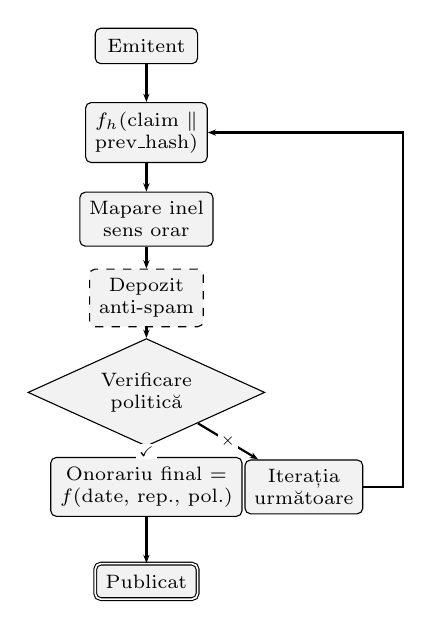
\begin{tikzpicture}[
    box/.style={draw, rounded corners=2pt, minimum width=1.3cm, minimum height=0.45cm, align=center, font=\scriptsize, fill=black!5},
    dec/.style={draw, diamond, aspect=2.2, minimum width=0.9cm, align=center, font=\scriptsize, fill=black!5},
    arr/.style={-{Stealth[length=3pt]}, thick},
    lbl/.style={font=\tiny, fill=white, inner sep=1pt}
]
\node[box] (iss) at (0,0) {Emitent};
\node[box] (hash) at (0,-1.1) {$f_h$(claim $\|$\\prev\_hash)};
\node[box] (ring) at (0,-2.2) {Mapare inel\\sens orar};
\node[box, dashed] (spam) at (0,-3.2) {Depozit\\anti-spam};
\node[dec] (check) at (0,-4.4) {Verificare\\politică};
\node[box] (rej) at (2,-5.6) {Iterația\\următoare};
\node[box] (fee) at (0,-5.6) {Onorariu final =\\$f$(date, rep., pol.)};
\node[box, double] (pub) at (0,-6.8) {Publicat};

\draw[arr] (iss) -- (hash);
\draw[arr] (hash) -- (ring);
\draw[arr] (ring) -- (spam);
\draw[arr] (spam) -- (check);
\draw[arr] (check) -- node[lbl] {$\times$} (rej);
\draw[arr] (check) -- node[lbl] {\checkmark} (fee);
\draw[arr] (fee) -- (pub);
\draw[arr] (rej.east) -- ++(0.5,0) |- (hash.east);
\end{tikzpicture}
\caption{Protocolul de selecție a verificatorului. Depozitul anti-spam este opțional și poate fi rambursabil. Onorariul final se plătește doar la acceptare.}
\label{fig:verifier}
\end{figure}

Fiecare respingere adaugă răspunsul complet al verificatorului (inclusiv motive și condiții) la documentul afirmației, extinzându-i conținutul. Din documentul extins, se calculează nedeterminist un nou hash, mapat pe o poziție diferită pe inel și selectând un verificator diferit. Documentarea căii complete este obligatorie---emitentul nu poate prezice sau influența verificatorul următor. Dacă un verificator ignoră o cerere în ciuda unei politici declarate compatibile, martorii (dacă sunt prezenți) înregistrează acest lucru, iar emitentul poate atașa dovezile martorilor la publicarea finală.

\begin{figure}[ht]
\centering
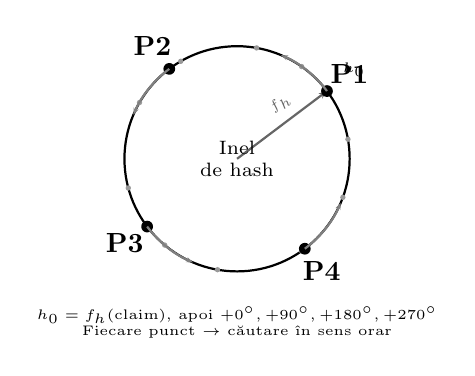
\begin{tikzpicture}[scale=0.65]
% Ring
\draw[thick] (0,0) circle (2.2cm);
% DID nodes on ring
\foreach \a in {10,55,80,120,150,195,230,260,305,340} {
  \fill[black!40] (\a:2.2) circle (1.5pt);
}
% Hash offset arrow pointing to initial position
\draw[-{Stealth[length=3pt]}, thick, black!60] (0,0) -- node[font=\tiny,above,sloped,pos=0.6] {$f_h$} (37:2.2);
\fill[black] (37:2.2) circle (2pt);
\node[font=\tiny,anchor=south west] at (37:2.35) {$h_0$};
% N=4 points offset from h0 by +0, +90, +180, +270
\foreach \offset/\l in {0/P1,90/P2,180/P3,270/P4} {
  \pgfmathsetmacro{\ang}{37+\offset}
  \node[fill=black, circle, inner sep=1.5pt] (p\offset) at (\ang:2.2) {};
  \node[font=\tiny,font=\bfseries] at (\ang:2.75) {\l};
  % clockwise search arc
  \draw[-{Stealth[length=2.5pt]}, thick, gray] (\ang:2.2) arc (\ang:\ang+30:2.2);
}
\node[font=\scriptsize, align=center] at (0,0) {Inel\\de hash};
\node[font=\tiny, align=center] at (0,-3.2) {$h_0 = f_h(\text{claim})$, apoi $+0^{\circ},+90^{\circ},+180^{\circ},+270^{\circ}$\\Fiecare punct $\rightarrow$ căutare în sens orar};
\end{tikzpicture}
\caption{Selecție cu puncte multiple ($N{=}4$). Hash-ul $h_0$ stabilește decalajul; 4 puncte distribuite uniform de la $h_0$.}
\label{fig:multipoint}
\end{figure}

\subsection{Protocolul martorului}

Rolul de \textbf{Martor} oferă responsabilizare incognito pentru onestitatea verificatorului printr-un protocol criptografic de cod de provocare:

\textbf{Pasul W1.} Solicitantul semnează cererea de verificare și o trimite către $N_w$ martori---contacte din rețeaua socială a solicitantului sau furnizori specializați de servicii de martor care operează contra cost.

\textbf{Pasul W2.} Fiecare martor $w_i$ semnează întreaga cerere semnată, păstrează semnătura originală $\sigma_i$ și calculează un cod de provocare $c_i = h(\sigma_i)$. Codul de provocare este adăugat la cerere.

\textbf{Pasul W3.} Cererea, purtând acum $N_w$ coduri de provocare, este trimisă către verificator. Verificatorul observă codurile, dar \emph{nu poate determina} cine sunt martorii sau dacă codurile corespund unor semnături reale.

\textbf{Pasul W4 (verificator onest).} Dacă verificatorul răspunde conform politicii sale declarate, codurile de provocare rămân opace. Martorii nu sunt niciodată dezvăluiți. Nu se publică date suplimentare.

\textbf{Pasul W5 (încălcare de politică).} Dacă verificatorul își încalcă politica (ignoră cererea, răspunde inconsecvent), solicitantul deține semnăturile originale ale martorilor $\sigma_i$. Acestea pot fi publicate ca date însoțitoare: oricine poate verifica $c_i = h(\sigma_i)$, demonstrând că martorul a fost prezent. Solicitantul poate publica independent---verificatorul a semnat deja codurile de provocare în răspunsul său.

\textbf{Proprietatea de cacealma.} Solicitantul poate înlocui unele sau toate codurile de provocare cu valori aleatorii. Verificatorul nu poate distinge codurile autentice (susținute de autorități cu reputație înaltă) de zgomot. Această \emph{incertitudine} este mecanismul de impunere: fiecare cerere poartă riscul ca o autoritate respectată să privească incognito. Costul menținerii acestei presiuni este aproape zero (generarea de numere aleatorii), în timp ce costul potențial al necinstei pentru verificator este catastrofal. Comportamentul onest este stimulat chiar și în absența martorilor reali.

\textbf{Autoritatea ca martor.} O Autoritate care avizează o afirmație poate combina serviciile de martor: „Avizez afirmația ta și servesc drept martor incognito în timpul verificării.” Acesta este un model de afaceri natural---Autoritatea are deja contextul. Totuși, cele două roluri sunt logic independente.

\subsection{Principiul Radicalismului Costisitor}

Trei canale de cost se compun simultan (Fig.~\ref{fig:radicalism}):

\textbf{Canalul 1: Costul iterației.} Fiecare respingere forțează o nouă iterație care consumă timp și resurse. Creștere liniară.

\textbf{Canalul 2: Umflarea documentului.} Fiecare iterație adaugă răspunsul complet al verificatorului la documentul afirmației. Creșterea este liniară, dar cu un decalaj de bază: încărcătura inițială (conținutul afirmației, avizarea autorității, semnăturile criptografice) are deja o dimensiune netrivială $B_0$. Dimensiunea totală după $k$ iterații: $S(k) = B_0 + k \cdot \Delta$, unde $\Delta$ este dimensiunea medie a răspunsului.

\textbf{Canalul 3: Prima de risc a verificatorului.} Riscul este subiectiv. Verificatorul evaluează dacă politicile declarate ale DID-ului solicitant intră în conflict cu propriile interese comerciale, sociale sau politice ale verificatorului. Prima poate escalada exponențial odată cu distanța percepută față de „idealul” verificatorului: $P(d) = \alpha \cdot e^{\beta d}$, unde $d$ este metrica de distanță subiectivă a verificatorului. Dincolo de o graniță personală interzisă, verificatorul poate refuza complet.

\begin{figure}[ht]
\centering
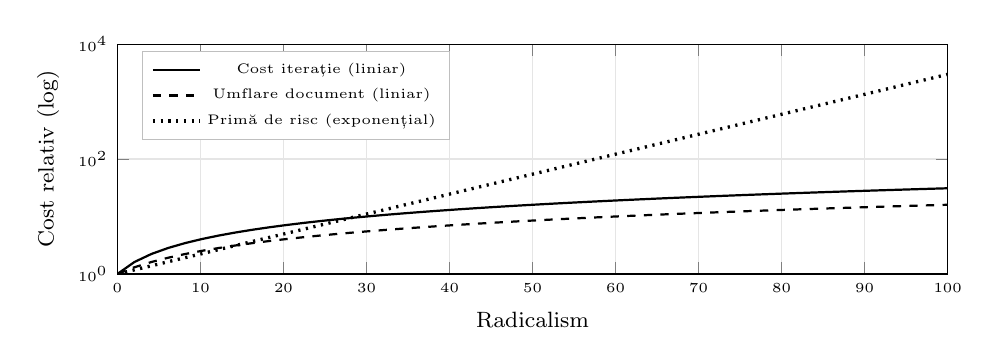
\begin{tikzpicture}
\begin{axis}[
    width=\columnwidth,
    height=4.5cm,
    xlabel={\footnotesize Radicalism},
    ylabel={\footnotesize Cost relativ (log)},
    ymode=log,
    xmin=0, xmax=100,
    ymin=1, ymax=10000,
    grid=major,
    grid style={gray!20},
    legend style={at={(0.03,0.97)},anchor=north west,font=\tiny,draw=gray!50},
    tick label style={font=\tiny},
    label style={font=\footnotesize},
]
\addplot[black, thick, domain=0:100, samples=50] {1 + 0.3*x};
\addlegendentry{Cost iterație (liniar)}
\addplot[black, thick, dashed, domain=0:100, samples=50] {1 + 0.15*x};
\addlegendentry{Umflare document (liniar)}
\addplot[black, thick, dotted, line width=1.2pt, domain=0:100, samples=100] {exp(0.08*x)};
\addlegendentry{Primă de risc (exponențial)}
\end{axis}
\end{tikzpicture}
\caption{Escaladarea costului pe trei canale. Prima de risc domină la radicalism ridicat.}
\label{fig:radicalism}
\end{figure}

În mod critic, aceasta nu este cenzură. Nicio afirmație nu este interzisă. Sistemul taxează riscul (Tabelul~\ref{tab:costs}).

\begin{table}[ht]
\centering
\caption{Comparație de cost între tipurile de afirmații.}
\label{tab:costs}
\footnotesize
\begin{tabular}{@{}lcccc@{}}
\toprule
\textbf{Tip} & \textbf{Iter.} & \textbf{Doc} & \textbf{Onor.} & \textbf{Total} \\
\midrule
Credibilă & $k_{\min}$ & $B_0$ & $P_{\min}$ & Scăzut \\
Controversată & $k_{\text{med}}$ & $B_0{+}k\Delta$ & $\alpha e^{\beta d}$ & Moderat \\
Radicală & $k_{\max}$ & $\gg B_0$ & $\gg P_{\min}$ & Foarte ridicat \\
Frauduloasă & $\to\infty$ & --- & --- & Nepublicabilă \\
\bottomrule
\end{tabular}
\end{table}

% ============================================================
% 6. REPUTATION AND RISK
% ============================================================
\section{Reputația și evaluarea riscului}

\subsection{Modelul de acumulare a reputației}

Reputația prezintă trei proprietăți: \textbf{acumulare lentă} (creștere incrementală prin comportament consistent), \textbf{distrugere rapidă} (o singură fraudă poate reduce scorul catastrofal) și \textbf{evaluare individuală} (fiecare parte consumatoare poate aplica propria funcție de agregare).

\subsection{Autorități Reputabile}

O Autoritate Reputabilă examinează afirmațiile și, dacă este mulțumită, le co-semnează---punându-și în joc propria reputație (Fig.~\ref{fig:authority}). Asimetria este intenționată: câștigarea reputației este lentă (incremental $+\delta$ per avizare onestă), în timp ce pierderea ei este catastrofală ($-\Delta \gg \delta$ per avizare falsă; ilustrativ, de ex., $+2\%$ față de $-70\%$). Strategia optimă este întotdeauna respingerea afirmațiilor suspecte. Valorile specifice ale $\delta$ și $\Delta$ sunt parametri ai sistemului.

\begin{figure}[ht]
\centering
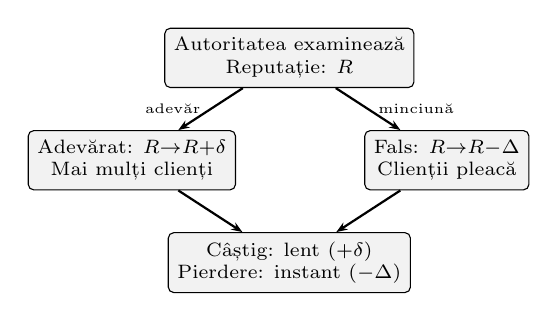
\begin{tikzpicture}[
    box/.style={draw, rounded corners=2pt, minimum width=2cm, minimum height=0.6cm, align=center, font=\scriptsize, fill=black!5},
    arr/.style={-{Stealth[length=4pt]}, thick}
]
\node[box] (exam) at (0,0) {Autoritatea examinează\\Reputație: $R$};
\node[box] (true) at (-2,-1.3) {Adevărat: $R{\to}R{+}\delta$\\Mai mulți clienți};
\node[box] (false) at (2,-1.3) {Fals: $R{\to}R{-}\Delta$\\Clienții pleacă};
\node[box] (insight) at (0,-2.6) {Câștig: lent ($+\delta$)\\Pierdere: instant ($-\Delta$)};

\draw[arr] (exam) -- node[left,font=\tiny] {adevăr} (true);
\draw[arr] (exam) -- node[right,font=\tiny] {minciună} (false);
\draw[arr] (true) -- (insight);
\draw[arr] (false) -- (insight);
\end{tikzpicture}
\caption{Autoritate Reputabilă---stimulente asimetrice.}
\label{fig:authority}
\end{figure}

\subsection{Reputație multidimensională}

Reputația nu este un scalar, ci un vector pe mai multe dimensiuni: fiabilitate financiară, integritate personală, competență profesională, angajament civic și altele (Fig.~\ref{fig:reputation-radar}). Diferiți furnizori de evaluare proiectează acest vector diferit, în funcție de context---un creditor prioritizează fiabilitatea financiară, un angajator competența profesională, un vecin comportamentul civic. Nu există un singur scor de reputație „corect”; doar perspective.

\begin{figure}[ht]
\centering
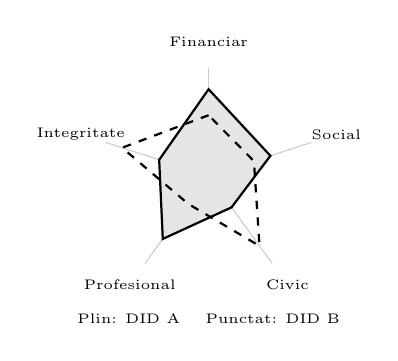
\begin{tikzpicture}[scale=0.55]
\foreach \a/\l in {90/Financiar,162/Integritate,234/Profesional,306/Civic,18/Social} {
  \draw[gray!40] (0,0) -- (\a:2.5);
  \node[font=\tiny, align=center] at (\a:3.1) {\l};
  \foreach \r in {0.8,1.6,2.4} {
    \fill[black!15] (\a:\r) circle (0.5pt);
  }
}
\draw[thick, fill=black!10] (90:2.0) -- (162:1.2) -- (234:1.8) -- (306:0.9) -- (18:1.5) -- cycle;
\draw[thick, dashed] (90:1.4) -- (162:2.1) -- (234:0.8) -- (306:2.0) -- (18:1.1) -- cycle;
\node[font=\tiny] at (0,-3.3) {Plin: DID A \quad Punctat: DID B};
\end{tikzpicture}
\caption{Vectori de reputație multidimensională. DID-uri diferite prezintă profiluri diferite pe dimensiuni.}
\label{fig:reputation-radar}
\end{figure}

\subsection{Evaluarea democratizată a riscului}

RSN democratizează evaluarea sistematică a riscului---o capacitate concentrată în prezent în instituțiile financiare, dar aplicabilă cu mult dincolo de domeniul bancar. Conglomerate industriale care evaluează fiabilitatea furnizorilor, companii de asigurări care taxează riscul comportamental, due diligence pentru fuziuni și achiziții, estimarea duratei de viață a echipamentelor în producție---oriunde riscul contrapărții necesită evaluare, RSN oferă o alternativă descentralizată, orientată spre piață. O piață de servicii de interpretare traduce datele brute de reputație multidimensională în rezumate acționabile, făcând evaluarea contrapărții accesibilă oricărui participant la cost marginal.

% ============================================================
% 7. CONSENSUS AND DISPUTE RESOLUTION
% ============================================================
\section{Consens și soluționarea disputelor}

\subsection{Modelul de justiție descentralizată}

RSN reformulează justiția ca o problemă de negociere bilaterală. Amenințarea unei deteriorări permanente și verificabile a reputației este un factor de descurajare mai eficient decât procesele judiciare pe care partea vătămată nu și le poate permite.

\subsection{Consens emergent}

Fiecare participant menține un prag personal de satisfacție. Consensul agregat al rețelei emerge ca media statistică a mii de negocieri bilaterale (Fig.~\ref{fig:consensus}). Un răspuns cu mult peste consens (barbar) este costisitor de publicat. Un răspuns aproape de consens (proporțional) este ieftin. Consensul nu este o regulă---este un semnal de preț.

\begin{figure}[ht]
\centering
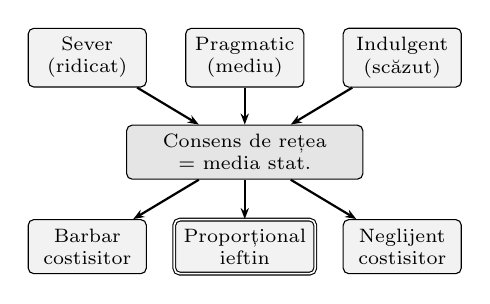
\begin{tikzpicture}[
    person/.style={draw, rounded corners=2pt, minimum width=1.5cm, minimum height=0.5cm, align=center, font=\scriptsize, fill=black!5},
    arr/.style={-{Stealth[length=4pt]}, thick}
]
\node[person] (a) at (-2,0) {Sever\\(ridicat)};
\node[person] (b) at (0,0) {Pragmatic\\(mediu)};
\node[person] (c) at (2,0) {Indulgent\\(scăzut)};
\node[person, fill=black!10, minimum width=3cm] (cons) at (0,-1.2) {Consens de rețea\\= media stat.};
\node[person] (exp) at (-2,-2.4) {Barbar\\costisitor};
\node[person, double] (prop) at (0,-2.4) {Proporțional\\ieftin};
\node[person] (neg) at (2,-2.4) {Neglijent\\costisitor};

\draw[arr] (a) -- (cons);
\draw[arr] (b) -- (cons);
\draw[arr] (c) -- (cons);
\draw[arr] (cons) -- (exp);
\draw[arr] (cons) -- (prop);
\draw[arr] (cons) -- (neg);
\end{tikzpicture}
\caption{Consens emergent din pragurile individuale de satisfacție.}
\label{fig:consensus}
\end{figure}

\subsection{Calibrarea pedepsei}

Fiecare Deținător de DID declară public răspunsurile la categorii specifice de rea conduită. Declarațiile disproporționat de aspre sau de indulgente atrag semnale de reputație negative. Declarațiile proporționale sunt acceptate fără fricțiune---un sistem de pedeapsă auto-calibrant.

Declarațiile de consens sunt ele însele supuse detectării ipocriziei: angajarea declarativă față de o poziție de consens comportându-se totodată inconsecvent constituie o abatere reputațională mai gravă decât abaterea de bază, deoarece demonstrează o înșelăciune intenționată.

\subsection{Delegarea}

Toate activitățile din cadrul unui DID---cu o singură excepție---pot fi delegate unui alt DID. \textbf{Rolul de Subiect---DID-ul despre al cărui comportament este afirmația---nu poate fi delegat; este legat netransferabil de deținătorul identității la care se referă afirmația.} Celelalte roluri active---Emitent, Autoritate, Martor, Verificator---pot fi transferate unui DID delegat desemnat, fie pentru verificare, trimiterea afirmației, participarea la consens sau soluționarea disputelor. Delegarea este revocabilă în orice moment. Aceasta permite specializarea (de ex., servicii profesionale de verificare) în timp ce Deținătorul păstrează controlul și responsabilitatea supreme. Delegarea se aplică în întregul sistem și este esențială pentru scalabilitate.

\subsection{De la moralitatea individuală la contractul social emergent}

Politica declarată a fiecărui DID reprezintă o formalizare a moralității individuale: ceea ce Deținătorul consideră acceptabil, cum răspunde la comportamente specifice, ce cere de la contrapărți. Aceste politici nu sunt impuse de un proiectant de sistem---ele sunt alese de fiecare participant și exprimate într-o formă care poate fi citită de mașini.

Această formalizare permite o emergență în trei etape. În primul rând, moralitatea individuală este codificată drept \textbf{politică}---un set de reguli declarate, praguri și funcții de răspuns pe care DID-ul se angajează să le urmeze. În al doilea rând, agregatul tuturor politicilor din rețea produce \textbf{etică emergentă}---norme observabile statistic pe care niciun participant nu le-a proiectat, dar care apar din interacțiunea a mii de poziții morale individuale~\cite{durkheim1893}. În al treilea rând, această etică emergentă, exprimată ca norme comportamentale comune impuse prin semnale bilaterale de preț, constituie un \textbf{contract social măsurabil}---nu un construct teoretic pe care nimeni nu l-a semnat~\cite{rawls1971}, ci un set de reguli observabil empiric, susținut de comportament real.

Acest proces reflectă concluziile teoriei fundamentelor morale~\cite{haidt2012}: moralitatea umană este intuitivă, pluralistă și variabilă cultural. RSN nu necesită consensul moral ca intrare; el produce consensul comportamental ca ieșire. Contractul social rezultat nu este static---el evoluează pe măsură ce participanții aderă, pleacă și își ajustează politicile ca răspuns la feedback-ul rețelei. Spre deosebire de teoria clasică a contractului social, acest contract este revocabil, observabil și aplicabil fără un suveran.

% ============================================================
% 8. ECONOMIC MODEL
% ============================================================
\section{Modelul economic}

Secțiunile precedente au descris un instrument---mecanismele de verificare ale RSN, structura costurilor și consensul emergent. Această secțiune descrie o metodologie de aplicare a acestui instrument la tranziția fiscală și de guvernare. Instrumentul este de uz general; metodologia de mai jos este o posibilă aplicație.

\subsection{Structura stimulentelor}

Reputația ca și capital creează stimulente directe pentru comportamentul onest. În funcționarea normală, participanții își construiesc reputația în mod natural prin tranzacții cotidiene și angajamente onorate. Cheltuiala principală este pentru afirmațiile \emph{negative}---înregistrarea prejudiciului cauzat de alții. Această asimetrie stimulează comportamentul util și fiabil: a fi onest nu costă nimic în plus, în timp ce a fi dăunător creează o urmă documentată pe care alții vor plăti să o păstreze. Ipocrizia---declararea de reguli fără a le urma---este cel mai costisitor mod de eșec, deoarece demonstrează o înșelăciune intenționată.

\subsection{Sistemul fiscal paralel}

Trei componente permit presiunea concurențială: (1)~\textbf{Impozit Simplu}---o singură cotă proporțională fără excepții, inițial marginal sub cota efectivă existentă; (2)~\textbf{Înregistrarea Electronică a Cheltuielilor (ESR)}---inversând modelul ceh EET astfel încât cetățenii să supravegheze cheltuielile statului; (3)~\textbf{Alocarea Impozitului Direcționată de Cetățean}---pornind de la câteva procente în primul an și ajungând, după un deceniu, oriunde de la un procent modest de două cifre până la o migrare completă către un sistem direcționat de cetățeni, în funcție de rata de adoptare. Tempo-ul efectiv depinde de viteza cu care apar alternative de piață liberă la serviciile statului și de disponibilitatea statului de a coopera cu tranziția; funcția de timp nu trebuie să fie liniară, iar nu există niciun motiv să se stabilească o limită superioară pentru punctul la care poate ajunge în cele din urmă adoptarea.

% ============================================================
% 9. MIGRATION PATH
% ============================================================
\section{Calea de migrare}

Migrarea se desfășoară în trei faze (Fig.~\ref{fig:migration}): \textbf{Faza~1: Suprapunere} (RSN ca strat informațional, statul este unicul furnizor), \textbf{Faza~2: Concurență} (RSN oferă alternative funcționale, utilizare a sistemului dublu) și \textbf{Faza~3: Tranziție} (RSN depășește echivalentele de stat, migrare voluntară). Tranziția este reversibilă în fiecare etapă.

\begin{figure}[ht]
\centering
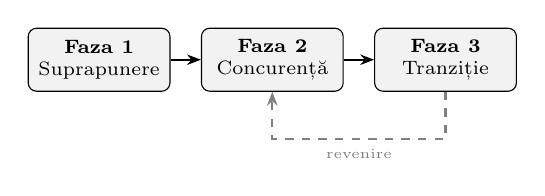
\begin{tikzpicture}[
    phase/.style={draw, rounded corners=3pt, minimum width=1.8cm, minimum height=0.8cm, align=center, font=\scriptsize, fill=black!5},
    arr/.style={-{Stealth[length=5pt]}, thick}
]
\node[phase] (p1) at (0,0) {\textbf{Faza 1}\\Suprapunere};
\node[phase] (p2) at (2.2,0) {\textbf{Faza 2}\\Concurență};
\node[phase] (p3) at (4.4,0) {\textbf{Faza 3}\\Tranziție};

\draw[arr] (p1) -- (p2);
\draw[arr] (p2) -- (p3);
\draw[arr, dashed, gray] (p3.south) -- ++(0,-0.6) -| node[below,font=\tiny,pos=0.25] {revenire} (p2.south);
\end{tikzpicture}
\caption{Migrare în trei faze---reversibilă în fiecare etapă.}
\label{fig:migration}
\end{figure}

Mecanismul principal de presiune este fiscal: când contribuabilii condiționali ating o „minoritate semnificativă economic $X$”---un grup suficient de mare încât represiunea împotriva lui să cauzeze pagube economice netriviale, iar nesupunerea civică să devină o amenințare credibilă---statul intră în negociere. Pentru ilustrare, folosim $X \approx 15\%$ din PIB, dar pragul efectiv depinde de economia specifică.

% ============================================================
% 10. SECURITY ANALYSIS
% ============================================================
\section{Analiza de securitate}

Considerăm cinci categorii de adversari: actori răuvoitori individuali, grupuri organizate, adversari corporativi, adversari la nivel de stat și adversari la nivel de protocol.

\textbf{Rezistență la atacuri Sybil}~\cite{douceur2002}. Construirea reputației necesită o interacțiune susținută și verificabilă. Costul unui atac Sybil reușit crește liniar cu numărul de identități false și cuadratic cu nivelul de reputație țintit. Operarea mai multor DID-uri în paralel este posibilă, dar costisitoare prin proiectare---fiecare identitate trebuie să își acumuleze independent reputația printr-o activitate autentică. În societățile libere, acest cost descurajează abuzul ocazional; în dictaturi, DID-urile paralele devin un instrument de supraviețuire care permite rezistența compartimentată, coordonarea din subteran și navigarea mai sigură pe piața neagră.

\textbf{Apărare împotriva coluziunii.} Tiparele de avizare reciprocă în cadrul grupurilor închise sunt detectabile prin analiza grafului social. Funcțiile de agregare a reputației reduc ponderea afirmațiilor provenite din surse strâns grupate.

\textbf{Adversar la nivel de stat.} Rutarea onion, absența infrastructurii centralizate și distribuirea rolului de Verificator în întreaga bază de participanți asigură faptul că suprimarea necesită măsuri disproporționate față de orice beneficiu.

\textbf{Confidențialitate vs.\ responsabilizare.} Pseudonimitatea---o cale de mijloc între anonimat și dezvăluirea identității---permite DID-urilor să acumuleze o reputație semnificativă fără a dezvălui identitatea reală a Deținătorului.

% ============================================================
% 11. PRIVACY
% ============================================================
\section{Considerații privind confidențialitatea}

Modelul de confidențialitate al RSN se bazează pe pseudonimitate. Deținătorul controlează dezvăluirea identității: minimă (pseudonim pur), selectivă (credențiale specifice legate) sau completă (identitate juridică asociată). Afirmațiile publicate sunt permanente---sistemul susține corectarea contextuală, dar nu ștergerea. Un Deținător poate abandona un DID compromis și porni de la zero, renunțând la reputația acumulată.

% ============================================================
% 12. RELATED WORK
% ============================================================
\section{Lucrări conexe}

Specificația W3C DID Core~\cite{did2022} și Ceramic Network~\cite{ceramic2023} oferă fundamentul de identitate. EigenTrust~\cite{kamvar2003} a demonstrat agregarea distribuită a reputației fără autoritate centrală. SBT-urile~\cite{weyl2022} au introdus token-uri sociale netransferabile. RSN diferă prin accentul pus pe costul economic ca filtru de calitate și prin mecanismul său de taxare a radicalismului.

DAO-urile~\cite{buterin2014} și votul cuadratic~\cite{buterin2019} au demonstrat fezabilitatea guvernării descentralizate. RSN derivă consensul din negocieri bilaterale de preț, mai degrabă decât din vot.

Propunerea se bazează pe teoria anarho-capitalistă~\cite{rothbard1973,hoppe2001} pentru furnizarea privată de servicii, dar se abate în două privințe critice: proiectează pentru ranchiună și impulsuri retributive, mai degrabă decât presupunând raționalitate, și propune o tranziție graduală, nu o revoluție. Conceptul de contracte sociale emergente are antecedente în teoria ordinii spontane a lui Hayek~\cite{hayek1973}.

\textbf{Anarho-agorism.} RSN împărtășește un teren comun semnificativ cu contra-economia agoristă~\cite{konkin2006}---în special accentul pe construirea de instituții paralele și schimbul voluntar. Totuși, agorismul tinde să presupună interesul propriu rațional ca mecanism suficient de coordonare și adesea îi lipsește o cale concretă de migrare de la structurile statale existente. RSN încorporează explicit tendințe comportamentale non-raționale și oferă un mecanism de presiune fiscală pentru tranziția graduală.

\textbf{Meritocrație.} RSN poate reprezenta o primă descriere funcțională a modului în care meritocrația~\cite{young1958} poate emerge ca o proprietate sistemică, mai degrabă decât ca un slogan. Sistemele meritocratice tradiționale eșuează pentru că necesită o autoritate centrală care să definească și să impună „meritul”. În RSN, meritul emerge din evaluări bilaterale: cei care oferă valoare acumulează reputație; niciun comitet nu decide cine are merit.

\textbf{Proprietatea ca privilegiu.} RSN se abate fundamental de la tratamentul anarho-capitalist și al școlii austriece al drepturilor de proprietate ca naturale și absolute. În cadrul RSN, proprietatea este un \emph{privilegiu}---o recunoaștere socială care poate, în cazuri extreme, să fie retrasă de comunitate atunci când un participant încalcă fundamental normele comune (trădare, refuzul de a apăra comunitatea într-o criză existențială, exploatare sistematică). Aceasta nu este expropriere de stat, ci o retragere a recunoașterii sociale de către rețeaua de relații bilaterale.

% ============================================================
% 13. LIMITATIONS
% ============================================================
\section{Discuție și limitări}

\textbf{Pornirea la rece.} Valoarea RSN depinde de efectele de rețea; cei care adoptă devreme se confruntă cu o valoare limitată până când participarea atinge un prag. Totuși, chiar și din stadiile timpurii, rețeaua DID servește drept sursă utilă de informație suplimentară. Se așteaptă ca evaluarea timpurie a reputației și estimarea autorității să se dezvolte treptat, cu o sofisticare crescândă.

\textbf{Anti-parazitism și control al accesului.} DID-urile țintă pot impune onorarii gradate și restricții de acces la interogările de la DID-uri cu reputație scăzută. Aceasta nu este binară, ci o scală continuă: cu cât un DID interogator are mai puțină reputație, cu atât primește mai puțină informație, așteaptă mai mult și plătește mai mult. Acest mecanism stimulează participarea autentică în locul consumului pasiv.

\textbf{Inegalitatea accesului.} Costul publicării afirmațiilor poate filtra plângeri legitime de la participanți dezavantajați economic. Atenuare: fiecare participant servește simultan drept potențial verificator (sau deleagă acest rol) și câștigă onorarii de verificare. Pe un orizont de timp suficient, un participant non-radical ar trebui să se apropie de neutralitatea financiară---venitul din verificare compensând aproximativ costurile de publicare. Aceasta este o așteptare statistică, nu o garanție.

\textbf{Inegalitatea reputației.} Cei care adoptă devreme acumulează avantaje care pot crea bariere pentru cei care vin mai târziu. Totuși, evaluarea reputației este efectuată de furnizori terți care pot alege să atenueze avantajul primului venit prin algoritmii lor de agregare. A fi primul cu o bună reputație este un avantaj economic comparativ legitim---și acest lucru este intenționat.

\textbf{Întrebări deschise.} Funcțiile optime de cost, standardele de agregare, guvernarea protocolului și interacțiunea cu datele de reputație sintetică generate de IA rămân domenii pentru lucrări viitoare.

Această lucrare nu pretinde că RSN va produce rezultate optime în toate circumstanțele. Ea pretinde că RSN reprezintă o alternativă \emph{fezabilă}---implementabilă tehnic, autosustenabilă economic și compatibilă social cu tendințele comportamentale umane așa cum sunt ele în realitate.

% ============================================================
% 14. CONCLUSION
% ============================================================
\section{Concluzie}

Această lucrare a prezentat Rețeaua Socială de Reputație, un protocol descentralizat care permite schimbul de reputație pseudonim și verificabil. Principiul Radicalismului Costisitor asigură faptul că afirmațiile frauduloase sunt scoase de pe piață prin preț, fără cenzură. Calea de migrare propusă permite o tranziție graduală și reversibilă de la instituțiile existente. Proiectarea încorporează natura umană așa cum este---inclusiv meschinăria, ranchiuna și dorința de satisfacție retributivă---mai degrabă decât să necesite o transformare ideologică. Rezultatul nu este o utopie, ci un sistem în care dreptatea este accesibilă, reputația este câștigată, iar costul relei conduite este suportat de partea care a cauzat-o.

% ============================================================
% REFERENCES
% ============================================================
\bibliography{references}

\end{document}
